\documentclass{plt}
\usetheme{metropolis}           % Use metropolis theme

\tikzset{double distance=1pt,>=latex}

\tikzset{
  parsetree/.style={
    level distance=2pc,
    sibling distance=1.8pc,
    every node/.style={fill=mBlue!15},
    every path/.style={thick},
    baseline=(current bounding box.west)
  }
}


\tikzset{
    mymodule/.style={draw, fill=white, drop shadow},
    code/.style={draw, fill=gray!15, drop shadow,minimum width=0},
    emph/.style={draw, fill=mBlue!15, drop shadow},
}


% Make | a mathrel symbol: improves alternation (a | b) spacing
\mathcode`\|="326A

\def\filled#1{\ifx#11mRed\else white\fi}

%\DeclareSymbolFont{operator}{OT1}{put}{m}{n}
%\DeclareSymbolFont{letters}{OT1}{put}{m}{it}

% For drawing arithmetic parse trees

\def\plus#1#2{node {\texttt{+}} child {#1} child {#2}}
\def\minus#1#2{node {\texttt{-}} child {#1} child {#2}}
\def\mult#1#2{node {\texttt{*}} child {#1} child {#2}}
\def\lit#1{node {#1}}

\tikzfading[name=fade down,
  top color=transparent!0,
  bottom color=transparent!100]

\tikzfading[name=fade up,
  bottom color=transparent!0,
  top color=transparent!100]

\newcommand{\pac}{\begin{tikzpicture}
    \draw [fill=black!30!mBlue!100] (2.12pt,2.12pt) arc
    (45:315:3pt) -- (0,0) -- cycle;
  \end{tikzpicture}
}

\if 0
\newcommand{\handle}[3]{
  \begin{tikzpicture}
    \node [inner sep=1pt] (n1) {$#1$};
    \node [inner sep=1pt,anchor=base west] (n2) at (n1.base east) {$#2$};
    \node [inner sep=1pt,anchor=base west] (n1) at (n2.base east) {$#3$};
    \begin{pgfonlayer}{background}
      \draw [mRed!70,line width=2pt,rounded corners]
      ($(n2.north east) + (1pt,1pt)$) --
      ($(n2.north west) + (-1pt,1pt)$) --
      ($(n2.south west) + (-1pt,-1pt)$) --
      ($(n2.south east) + (1pt,-1pt)$) -- cycle
      ;
    \end{pgfonlayer}
  \end{tikzpicture}
}
\fi

\newcommand{\expand}[3]{
    \fill [even odd rule,mRed,path fading=fade up]
    (#1.north west)  [rounded corners] -- (#1.south west) --
    (#2.north west) -- (#2.south west) -- (#3.south east) --
    (#3.north east) -- (#1.south east) -- (#1.north east)
    -- cycle
    ($(#3.north east) + (-1pt,-1pt)$) --
    ($(#2.north west) + (1pt,-1pt)$) --
    ($(#2.south west) + (1pt,1pt)$) --
    ($(#3.south east) + (-1pt,1pt)$) -- cycle
    ;
}

\newcommand{\expandup}[3]{
    \fill [even odd rule,mRed,path fading=fade down]
    (#1.south west)  [rounded corners] -- (#1.north west) --
    (#2.south west) -- (#2.north west) -- (#3.north east) --
    (#3.south east) -- (#1.north east) -- (#1.south east)
    -- cycle
    ($(#3.south east) + (-1pt,1pt)$) --
    ($(#2.south west) + (1pt,1pt)$) --
    ($(#2.north west) + (1pt,-1pt)$) --
    ($(#3.north east) + (-1pt,-1pt)$) -- cycle
    ;
}



\newcommand{\id}{\textbf{Id}}

\newcommand{\grammarone}{
\renewcommand{\arraystretch}{1}
$\begin{array}[t]{@{}l@{\,}r@{\,}c@{\,}l@{}}
1: & e & \rightarrow & t + e \\
2: & e & \rightarrow & t \\
3: & t & \rightarrow & \id\ * t \\
4: & t & \rightarrow & \id
\end{array}$
}


\newenvironment{parsermoves}{
\begingroup
\small
\renewcommand{\arraystretch}{0.8}
\newcommand{\s}[2]{%
  \begin{pspicture}(10pt,10pt)
    \psframe(0,-5pt)(8pt,5pt)
    \rput(4pt,2pt){\tiny##1}
    \rput(4pt,-2pt){\tiny##2}
  \end{pspicture}}
\begin{tabular}[t]{l@{}rl}
\multicolumn{1}{c}{\hbox to 5em{\hss stack\hss}} & \multicolumn{1}{c}{input}
& \multicolumn{1}{c}{action} \\
}{
\end{tabular}
\endgroup
}


\title{Parser I}
\author{Ronghui Gu}
\institute{Columbia University}
\date{Spring 2019}
\titlegraphic{
\vspace{220pt}
{\tiny $^*$ Course website: \url{https://www.cs.columbia.edu/~rgu/courses/4115/spring2019}\vspace{-5pt}}\\
{\tiny $^{**}$ These slides are borrowed from Prof. Edwards.}
}

\begin{document}

\frame{\titlepage}

\part{The Big Picture}

\begin{frame}{The First Question}
  \begin{center}
    \large How do we describe/construct a program?
%    \vspace{5pc}
%
%    \emph{Compilers should accept many programs; \\
%      how do we describe which one we want?}
  \end{center}
\end{frame}

\begin{frame}{Solution: Use a Discrete Combinatorial System}

Use \emph{combinations} of a \emph{small number of things} to
represent (exponentially) many different things.

\begin{minipage}{0.2\textwidth}
\includegraphics[width=\textwidth]{dna-overview-clean.png}
\end{minipage}%
\begin{minipage}{0.8\textwidth}
\hfill
\includegraphics[width=0.3\textwidth]{rosetta-stone.jpg} \hfill
\includegraphics[width=0.5\textwidth]{English-sounds.png}

\hfill
\includegraphics[width=0.4\textwidth]{cells.jpg}
\hfill
\includegraphics[width=0.4\textwidth]{silicon-atoms.jpg}
\end{minipage}

\end{frame}

\begin{frame}{The Second Question}
  \begin{center}
    \large How do we combine \alert{characters} into \alert{words}? 

  \end{center}
\end{frame}



\begin{frame}[fragile,t]{Scanner}

\begin{center}
\hspace{20pt}
\begin{tikzpicture}
  \matrix [matrix of nodes,
           row sep=0.8pc,
           column sep=2pc,
           every node/.style={draw, fill=white, drop shadow,minimum width=5.5cm}] {
     |[code] (b)| int avg (int a, int b) ... \\
     |[emph] (a)| Lexical Analysis \\
     | (aa)| Syntax  Analysis \\
     |(aaa)| Semantic Analysis \\
     |(a4)| Intermediate Code Generation \\
     |(a5)| Optimization \\
     |(a6)| Code Generation \\
    |[code] (c)| 0101110101... \\
  };
  \begin{scope}[->]
    \draw (b) -- (a);
    \draw (a) -- (aa);
    \draw (aa) -- (aaa);
    \draw (aaa) -- (a4);
    \draw (a4) -- (a5);
    \draw (a5) -- (a6);
    \draw (a6) -- (c);
  \end{scope};
  \begin{scope}[densely dotted]
    \draw (-10pc,-2.6pc) -- (10pc,-2.6pc);
    \draw (-10pc,-5pc) -- (10pc,-5pc);
  \end{scope};
  \node at (9pc,0) {front-end};
  \node at (9.5pc,-4pc) {middle-end};
  \node at (9pc,-6pc) {back-end};
\end{tikzpicture}
\end{center}

\end{frame}

\begin{frame}{The Third Question}
  \begin{center}
    \large How do we combine \alert{words} into \alert{sentences}?
  \end{center}
\end{frame}



\begin{frame}[fragile,t]{Parser}

\begin{center}
\hspace{20pt}
\begin{tikzpicture}
  \matrix [matrix of nodes,
           row sep=0.8pc,
           column sep=2pc,
           every node/.style={draw, fill=white, drop shadow,minimum width=5.5cm}] {
     |[code] (b)| int avg (int a, int b) ... \\
     | (a)| Lexical Analysis \\
     | [emph] (aa)| Syntax  Analysis \\
     |(aaa)| Semantic Analysis \\
     |(a4)| Intermediate Code Generation \\
     |(a5)| Optimization \\
     |(a6)| Code Generation \\
    |[code] (c)| 0101110101... \\
  };
  \begin{scope}[->]
    \draw (b) -- (a);
    \draw (a) -- (aa);
    \draw (aa) -- (aaa);
    \draw (aaa) -- (a4);
    \draw (a4) -- (a5);
    \draw (a5) -- (a6);
    \draw (a6) -- (c);
  \end{scope};
  \begin{scope}[densely dotted]
    \draw (-10pc,-2.6pc) -- (10pc,-2.6pc);
    \draw (-10pc,-5pc) -- (10pc,-5pc);
  \end{scope};
  \node at (9pc,0) {front-end};
  \node at (9.5pc,-4pc) {middle-end};
  \node at (9pc,-6pc) {back-end};
\end{tikzpicture}
\end{center}

\end{frame}


\begin{frame}{Choices: CS Research Jargon Generator}

\begin{center}

Pick one from each column
\medskip

\begin{tabular}{lll}
\cmidrule(lr){1-1}
\cmidrule(lr){2-2}
\cmidrule(lr){3-3}
an integrated    & mobile          & network        \\
a parallel       & functional      & preprocessor   \\
a virtual        & programmable    & compiler       \\
an interactive   & distributed     & system         \\
a responsive     & logical         & interface      \\
a synchronized   & digital         & protocol       \\
a balanced       & concurrent      & architecture   \\
a virtual        & knowledge-based & database       \\
a meta-level     & multimedia      & algorithm      \\
\cmidrule(lr){1-1}
\cmidrule(lr){2-2}
\cmidrule(lr){3-3}
\end{tabular}

\medskip

E.g., ``a responsive knowledge-based preprocessor.''

\tiny
http://www.cs.purdue.edu/homes/dec/essay.topic.generator.html
\end{center}
\end{frame}


\begin{frame}
\centerline{\includegraphics[width=0.5\textwidth]{hey-jude-flowchart.jpg}}

\footnotesize http://loveallthis.tumblr.com/post/506873221
\end{frame}

\begin{frame}[fragile]{How about more structured collections of things?}

The boy eats hot dogs.

The dog eats ice cream.

Every happy girl eats candy.

A dog eats candy.

The happy happy dog eats hot dogs.

\begin{tikzpicture}[node distance=0.5pc and 2pc]
  \node [text width=2.5pc] (s1) {The \break A \break Every};
  \node [above right=of s1] (s2) {happy};
  \node [text width=2pc,below right=of s2] (s3) {boy\break girl\break dog};
  \node [right=of s3] (s4) {eats};
  \node [text width=4pc,right=of s4] (s5) {hot dogs.\break ice cream.\break candy.};
  \path [->]
    (s1) edge (s2)
    (s2) edge [loop above] ()
    (s2) edge (s3)
    (s1) edge (s3)
    (s3) edge (s4)
    (s4) edge (s5)
  ;
\end{tikzpicture}

\tiny Pinker, \emph{The Language Instinct}

\end{frame}

\begin{frame}{Richer Sentences Are Harder}

  If the boy eats hot dogs, then the girl eats ice cream.

  Either the boy eats candy, or every dog eats candy.


\begin{tikzpicture}[node distance=0.5pc and 1pc]
  \node [text width=2pc] (s0) {Either\break If};
  \node [text width=2.5pc,right=of s0] (s1) {the \break a \break every};
  \node [above right=of s1] (s2) {happy};
  \node [text width=1.8pc,below right=of s2] (s3) {boy\break girl\break dog};
  \node [right=of s3] (s4) {eats};
  \node [text width=4pc,right=of s4] (s5) {hot dogs\break ice cream\break candy};
  \node [text width=2pc,right=of s5] (s6) {or\break then};
  \path [->]
    (s0) edge (s1)
    (s1) edge (s2)
    (s2) edge [loop above] ()
    (s2) edge (s3)
    (s1) edge (s3)
    (s3) edge (s4)
    (s4) edge (s5)
    (s5) edge (s6)
    (s6) edge [bend left=80,looseness=0.4] (s1);
  ;
\end{tikzpicture}

\centerline{\emph{Does this work?}}

\end{frame}

\begin{frame}{Automata Have Poor Memories}

Want to ``remember'' whether it is an ``either-or'' or ``if-then''
sentence.  Only solution: duplicate states.

\tiny

\begin{tikzpicture}[node distance=0.3pc and 0.5pc]
  \node (s0) {};
  \node at (1pc,2pc) (sa0) {Either};
  \node [text width=1.5pc,right=of sa0] (sa1) {the \break a \break every};
  \node [above right=of sa1] (sa2) {happy};
  \node [text width=1.2pc,below right=of sa2] (sa3) {boy\break girl\break dog};
  \node [right=of sa3] (sa4) {eats};
  \node [text width=2.5pc,right=of sa4] (sa5) {hot dogs\break ice cream\break candy};
  \node [right=of sa5] (sa6) {or};
  \path [->]
    (sa0) edge (sa1)
    (sa1) edge (sa2)
    (sa2) edge [loop above] ()
    (sa2) edge (sa3)
    (sa1) edge (sa3)
    (sa3) edge (sa4)
    (sa4) edge (sa5)
    (sa5) edge (sa6);

  \node at (1pc,-2pc) (sb0) {If};
  \node [text width=1.5pc,right=of sb0] (sb1) {the \break a \break every};
  \node [above right=of sb1] (sb2) {happy};
  \node [text width=1.2pc,below right=of sb2] (sb3) {boy\break girl\break dog};
  \node [right=of sb3] (sb4) {eats};
  \node [text width=2.5pc,right=of sb4] (sb5) {hot dogs\break ice cream\break candy};
  \node [right=of sb5] (sb6) {then};
  \path [->]
    (s0) edge (sa0)
    (s0) edge (sb0)
    (sb0) edge (sb1)
    (sb1) edge (sb2)
    (sb2) edge [loop above] ()
    (sb2) edge (sb3)
    (sb1) edge (sb3)
    (sb3) edge (sb4)
    (sb4) edge (sb5)
    (sb5) edge (sb6);

  \node [text width=1.5pc] at (16pc,0pc) (sc1) {the \break a \break every};
  \node [above right=of sc1] (sc2) {happy};
  \node [text width=1.2pc,below right=of sc2] (sc3) {boy\break girl\break dog};
  \node [right=of sc3] (sc4) {eats};
  \node [text width=2.5pc,right=of sc4] (sc5) {hot dogs\break ice cream\break candy};
  \path [->]
    (sa6) edge (sc1)
    (sb6) edge (sc1)
    (sc1) edge (sc2)
    (sc2) edge [loop above] ()
    (sc2) edge (sc3)
    (sc1) edge (sc3)
    (sc3) edge (sc4)
    (sc4) edge (sc5);

\end{tikzpicture}

\end{frame}

\def\s#1{\hfil$#1:$\hfil\break}
\begin{frame}{Automata in the form of Production Rules}

Problem: automata do not remember where they've been

{\footnotesize\ttfamily
\begin{tabular}{l}
$S \rightarrow$ Either    $A$ \\
$S \rightarrow$ If        $A$ \\
$A \rightarrow$ the       $B$ \\
$A \rightarrow$ the       $C$ \\
$A \rightarrow$ a         $B$ \\
$A \rightarrow$ a         $C$ \\
$A \rightarrow$ every     $B$ \\
$A \rightarrow$ every     $C$ \\
$B \rightarrow$ happy     $B$ \\
$B \rightarrow$ happy     $C$ \\
$C \rightarrow$ boy       $D$ \\
$C \rightarrow$ girl      $D$ \\
$C \rightarrow$ dog       $D$ \\
$D \rightarrow$ eats      $E$ \\
$E \rightarrow$ hot dogs  $F$ \\
$E \rightarrow$ ice cream $F$ \\
$E \rightarrow$ candy     $F$ \\
$F \rightarrow$ or        $A$ \\
$F \rightarrow$ then      $A$ \\
$F \rightarrow$ $\epsilon$ \\
\end{tabular}}
\tiny
\begin{tikzpicture}[node distance=0.3pc and 0.5pc,
  every node/.style={draw}]
  \node [text width=1.5pc] (s0) {\s S Either\break If};
  \node [text width=1.5pc,right=of s0] (s1) {\s A the \break a \break every};
  \node [above right=of s1] (s2) {\s B happy};
  \node [text width=1.2pc,below right=of s2] (s3) {\s C boy\break girl\break dog};
  \node [right=of s3] (s4) {\s D eats};
  \node [text width=2.5pc,right=of s4] (s5) {\s E hot dogs\break ice cream\break candy};
  \node [text width=1.5pc,right=of s5] (s6) {\s F or\break then};
  \path [->]
    (s0) edge (s1)
    (s1) edge (s2)
    (s2) edge [loop above] ()
    (s2) edge (s3)
    (s1) edge (s3)
    (s3) edge (s4)
    (s4) edge (s5)
    (s5) edge (s6)
    (s6) edge [bend left=80,looseness=0.4] (s1);
  ;
\end{tikzpicture}

\end{frame}

\begin{frame}{Solution: Context-Free Grammars}

Context-Free Grammars have the ability to ``call subroutines:''

{\ttfamily
\begin{tabular}{ll}
$S \rightarrow$ Either $P$, or $P$. & \rmfamily \alert{Exactly two $P$s}\\
$S \rightarrow$ If $P$, then $P$. \\
$P \rightarrow$ $A$ $H$ $N$ eats $O$ & \rmfamily \alert{One each of $A$, $H$, $N$, and
    $O$} \\
$A \rightarrow$ the \\
$A \rightarrow$ a \\
$A \rightarrow$ every \\
$H \rightarrow$ happy $H$ & \rmfamily \alert{$H$ is ``happy'' zero or more times} \\
$H \rightarrow$ $\epsilon$ \\
$N \rightarrow$ boy \\
$N \rightarrow$ girl \\
$N \rightarrow$ dog \\
$O \rightarrow$ hot dogs \\
$O \rightarrow$ ice cream \\
$O \rightarrow$ candy \\
\end{tabular}
}

\end{frame}

\def\tok#1{\textbf{\texttt{#1}}}
%
%\begin{frame}{A Context-Free Grammar for a Simplified C}
%\small
%\[
%\begin{array}{r@{\hspace{3pt}}c@{\hspace{3pt}}l}
%\textit{program} & \rightarrow & \epsilon |
%   \textit{program}\ \textit{vdecl} |
%   \textit{program}\ \textit{fdecl} \\[5pt]
%\textit{fdecl} & \rightarrow &
%\tok{id}\ \tok{(}\ \textit{formals}\ \tok{)}\ \tok{\{}\ \textit{vdecls}\ \textit{stmts}\ \tok{\}}
%\\[5pt]
%\textit{formals} & \rightarrow & \tok{id} |
%\textit{formals}\ \tok{,}\ \tok{id} \\[5pt]
%\textit{vdecls} & \rightarrow & \textit{vdecl} | \textit{vdecls}\ \textit{vdecl} \\[5pt]
%\textit{vdecl} & \rightarrow & \tok{int}\ \tok{id}\ \tok{;} \\[5pt]
%\textit{stmts} & \rightarrow & \epsilon | \textit{stmts}\ \textit{stmt} \\[5pt]
%\textit{stmt} & \rightarrow & \textit{expr}\ \tok{;} |
%\tok{return}\ \textit{expr}\ \tok{;} |
%\tok{\{}\ \textit{stmts}\ \tok{\}} |
%\tok{if}\ \tok{(}\ \textit{expr}\ \tok{)}\ \textit{stmt} | \\&&
%\tok{if}\ \tok{(}\ \textit{expr}\ \tok{)}\ \textit{stmt}\ \tok{else}\ \textit{stmt}
%| \\&&
%\tok{for}\ \tok{(}\ \textit{expr}\ \tok{;}\ \textit{expr}\ \tok{;}\ \textit{expr}\ \tok{)}\ \textit{stmt}
%|
%\tok{while}\ \tok{(}\ \textit{expr}\ \tok{)}\ \textit{stmt}
%\\[5pt]
%\textit{expr} & \rightarrow &
%\tok{lit} | \tok{id} |
%\tok{id}\ \tok{(}\ \textit{actuals}\ \tok{)} |
%\tok{(}\ \textit{expr}\ \tok{)} | \\&&
%\textit{expr}\ \tok{+}\ \textit{expr} |
%\textit{expr}\ \tok{-}\ \textit{expr} |
%\textit{expr}\ \tok{*}\ \textit{expr} |
%\textit{expr}\ \tok{/}\ \textit{expr} | \\&&
%\textit{expr}\ \tok{==}\ \textit{expr} |
%\textit{expr}\ \tok{!=}\ \textit{expr} |
%\textit{expr}\ \tok{<}\ \textit{expr} |
%\textit{expr}\ \tok{<=}\ \textit{expr} |  \\&&
%\textit{expr}\ \tok{>}\ \textit{expr} |
%\textit{expr}\ \tok{>=}\ \textit{expr} |
%\textit{expr}\ \tok{=}\ \textit{expr}
%\\[5pt]
%\textit{actuals} & \rightarrow & \textit{expr} | \textit{actuals}
%\tok{,} \textit{expr} \\
%\end{array}
%\]
%
%\end{frame}


\begin{frame}{An Example}

\emph{n 0's followed by n 1's,} e.g., 000111, 01
\vspace{40pt}

{\ttfamily
\begin{tabular}{ll}
$S \rightarrow$ 0 $S$ 1. \\ 
$S \rightarrow$ $\epsilon$. 
\end{tabular}
}

\end{frame}

\part{Constructing Grammars and Ocamlyacc}
%\frame{\partpage}

\begin{frame}{Parsing}
Objective: build an abstract syntax tree (AST) for the token sequence
from the scanner.

\begin{center}
\texttt{2 * 3 + 4} \hspace{3pc} $\Rightarrow$ \hspace{3pc}
\begin{tikzpicture}[parsetree]
  \path \plus{\mult{\lit2}{\lit3}}{\lit4};
\end{tikzpicture}
\end{center}

\medskip

Goal: verify the syntax of the program, discard irrelevant
information, and ``understand'' the structure of the program.

Parentheses and most other forms of punctuation removed.

\end{frame}

\begin{frame}{Ambiguity in English}

\centerline{\emph{I shot an elephant in my pajamas}}

\begin{minipage}{0.35\textwidth}
\footnotesize
\begin{tabular}{@{}>{\itshape}l>{$}c<{$}>{\itshape}l@{}}
S & \rightarrow & NP VP \\
VP & \rightarrow & V NP \\
VP & \rightarrow & V NP PP \\
NP & \rightarrow & NP PP \\
NP & \rightarrow & Pro \\
NP & \rightarrow & Det Noun \\
NP & \rightarrow & Poss Noun \\
PP & \rightarrow & P NP \\
V & \rightarrow & \upshape shot \\
Noun & \rightarrow & \upshape elephant \\
Noun & \rightarrow & \upshape pajamas \\
Pro & \rightarrow & \upshape I \\
Det & \rightarrow & \upshape an \\
P & \rightarrow & \upshape in \\
Poss & \rightarrow & \upshape my \\
\end{tabular}
\end{minipage}%
\begin{minipage}{0.3\textwidth}
\tiny\itshape
  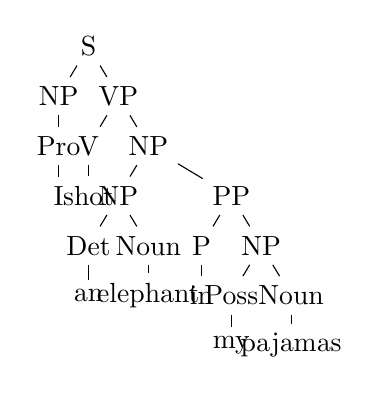
\begin{tikzpicture}[level distance=1.5pc,sibling distance=1.8pc]
    \node {S}
      child {node {NP}
        child {node {Pro}
          child {node {\upshape I}}
        }
      }
      child {node {\alert{VP}}
        child {node {V} child {node {\upshape shot}}}
        child {node {NP}
          child {node {NP}
            child {node {Det} child {node {\upshape an}}}
            child {node {Noun} child {node {\upshape elephant}}}
          }
          child [sibling distance=5pc] {node {PP}
            child [sibling distance=1.8pc] {node {P} child {node {\upshape in}}}
            child [sibling distance=1.8pc] {node {NP}
              child {node {Poss} child {node {\upshape my}}}
              child {node {Noun} child {node {\upshape pajamas}}}
            }
          }
        }
      }
    ;
  \end{tikzpicture}
\end{minipage}%
\begin{minipage}{0.3\textwidth}
\tiny\itshape
  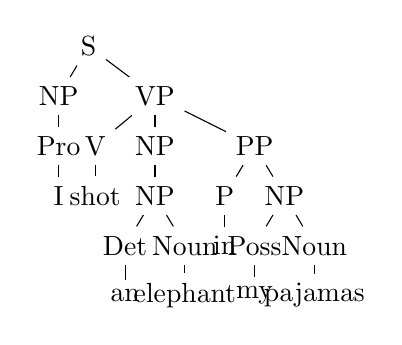
\begin{tikzpicture}[level distance=1.5pc,sibling distance=1.8pc]
    \node {S}
      child {node {NP}
        child {node {Pro}
          child {node {\upshape I}}
        }
      }
      child [sibling distance=4pc] {node {\alert{VP}}
        child [sibling distance=1.8pc] {node {V} child {node {\upshape shot}}}
        child [sibling distance=1.8pc] {node {NP}
          child {node {NP}
            child {node {Det} child {node {\upshape an}}}
            child {node {Noun} child {node {\upshape elephant}}}
          }
        }
        child [sibling distance=3pc] {node {PP}
          child [sibling distance=1.8pc] {node {P} child {node {\upshape in}}}
          child [sibling distance=1.8pc] {node {NP}
            child {node {Poss} child {node {\upshape my}}}
            child {node {Noun} child {node {\upshape pajamas}}}
          }
        }
      }
    ;
  \end{tikzpicture}
\end{minipage}

\tiny Jurafsky and Martin, \emph{Speech and Language Processing}

\end{frame}

\begin{frame}[fragile]{The Dangling Else Problem}

Who owns the \emph{else}?

\begin{center}\ttfamily
if (a) if (b) c(); else d();
\end{center}

\begin{ocamlyacc}
stmt : IF expr THEN stmt
     | IF expr THEN stmt ELSE stmt
\end{ocamlyacc}

Problem comes after matching the first statement.  Question is whether
an ``else'' should be part of the current statement or a surrounding
one since the second line tells us ``stmt ELSE'' is possible.

\end{frame}

\begin{frame}{The Dangling Else Problem}

\hfil
Should this be
\hfil
\begin{tikzpicture}[parsetree]
  \node {\texttt{if}}
     child {node {\texttt{a}}}
     child {node {\texttt{if}}
       child {node {\texttt{b}}}
       child {node {\texttt{c()}}}
       child {node {\texttt{d()}}}
     }
  ;
\end{tikzpicture}
\hfil
or
\hfil
\begin{tikzpicture}[parsetree]
  \node {\texttt{if}}
     child {node {\texttt{a}}}
     child {node {\texttt{if}}
       child {node {\texttt{b}}}
       child {node {\texttt{c()}}}
     }
     child {node {\texttt{d()}}}
  ;
\end{tikzpicture}
\hfil
?

Grammars are usually ambiguous; manuals give disambiguating rules such 
as C's:

\begin{quotation}
\noindent
As usual the ``else'' is resolved by connecting
an else with the last encountered elseless if.
\end{quotation}


\end{frame}


\begin{frame}[fragile]{The Dangling Else Problem}

Idea: break into two types of statements: those that have a dangling
``then'' (``dstmt'') and those that do not (``cstmt'').  A statement may be
either, but the statement just before an ``else'' must not have a
dangling clause because if it did, the ``else'' would belong to it.

\begin{ocamlyacc}
stmt : dstmt
     | cstmt

dstmt : IF expr THEN stmt
      | IF expr THEN cstmt ELSE dstmt

cstmt : IF expr THEN cstmt ELSE cstmt
      | other statements...
\end{ocamlyacc}

\begin{center}\ttfamily
if (a) if (b) c(); else d();
\end{center}
\end{frame}

\begin{frame}[fragile]{Another Solution to the Dangling Else Problem}
We are effectively carrying an extra bit of information during
parsing: whether there is an open ``then'' clause.  Unfortunately,
duplicating rules is the only way to do this in a context-free grammar.

\end{frame}


\begin{frame}[fragile]{Another Solution  to the Dangling Else Problem}

Some languages resolve this problem by insisting on nesting
everything.

E.g., Algol 68:

\begin{center}
\begin{algol}
if a < b then a else b fi;
\end{algol}
\end{center}

``fi'' is ``if'' spelled backwards.  The language also uses do--od and
case--esac.
\end{frame}

\begin{frame}{Ambiguous Arithmetic}

Ambiguity can be a problem in expressions.  Consider parsing

\begin{center}
\texttt{3 - 4 * 2 + 5}
\end{center}

with the grammar

\[e \rightarrow  e + e | e - e | e * e | e \mathop{/} e | N\]

\ttfamily

\begin{tikzpicture}[parsetree]
  \path
    \plus{\minus{\lit3}
                {\mult{\lit4}{\lit2}}}
         {\lit5}
    ;
\end{tikzpicture}
\hfil
\begin{tikzpicture}[parsetree]
  \path
    \minus{\lit3}
          {\plus{\mult{\lit4}{\lit2}}
                {\lit5}}
    ;
\end{tikzpicture}
\hfil
\begin{tikzpicture}[parsetree,
                 level 1/.style={sibling distance=3pc},
                 level 2/.style={sibling distance=1.8pc}]
  \path \mult{\minus{\lit3}{\lit4}}
              {\plus{\lit2}{\lit5}}
    ;
\end{tikzpicture}
\hfil
\begin{tikzpicture}[parsetree]
  \path \minus{\lit3}
              {\mult{\lit4}
                     {\plus{\lit2}{\lit5}}};
\end{tikzpicture}
\begin{tikzpicture}[parsetree]
  \path \minus{\mult{\plus{\lit3}{\lit4}}{\lit2}}{\lit5};
\end{tikzpicture}


\end{frame}

\begin{frame}{Operator Precedence and Associativity}

Usually resolve ambiguity in arithmetic expressions

Like you were taught in elementary school:

``My Dear Aunt Sally''

Mnemonic for multiplication and division before addition and subtraction.

\end{frame}

\begin{frame}{Operator Precedence}

Defines how ``sticky'' an operator is.

\begin{center}\ttfamily
1 * 2 + 3 * 4
\end{center}

\begin{minipage}{0.65\textwidth}
\texttt{*} at higher precedence than \texttt{+}:

\medskip

\texttt{(1 * 2) + (3 * 4)}
\end{minipage}
\begin{tikzpicture}[parsetree,
    level 1/.style={sibling distance=4pc},
    level 2/.style={sibling distance=2pc}]
  \path
  \plus{\mult{\lit1}{\lit2}}
       {\mult{\lit3}{\lit4}};
\end{tikzpicture}

\begin{minipage}{0.65\textwidth}
\texttt{+} at higher precedence than \texttt{*}:

\medskip

\texttt{1 * (2 + 3) * 4}
\end{minipage}
\begin{tikzpicture}[parsetree]
  \path
  \mult{\mult{\lit1}
               {\plus{\lit2}{\lit3}}}
        {\lit4};
\end{tikzpicture}
\end{frame}

\begin{frame}{Associativity}

Whether to evaluate left-to-right or right-to-left

Most operators are left-associative

\begin{center}
\texttt{1 - 2 - 3 - 4}

\vspace{2pc}

\begin{tabular}{c@{\hspace{5pc}}c}
  \ttfamily
  \begin{tikzpicture}[parsetree]
    \path \minus{\minus{\minus{\lit1}{\lit2}}{\lit3}}{\lit4};
  \end{tikzpicture}
&
  \ttfamily
  \begin{tikzpicture}[parsetree]
    \path \minus{\lit1}{\minus{\lit2}{\minus{\lit3}{\lit4}}};
  \end{tikzpicture}
\\
\\
$((1 - 2) - 3) - 4$ & $1 - (2 - (3 - 4))$ \\
\\
left associative & right associative
\end{tabular}

\end{center}

\end{frame}

\begin{frame}[fragile]{Fixing Ambiguous Grammars}

A grammar specification:

\begin{ocamlyacc}
expr :
    expr PLUS expr  
  | expr MINUS expr 
  | expr TIMES expr 
  | expr DIVIDE expr
  | NUMBER          
\end{ocamlyacc}

Ambiguous: no precedence or associativity.

Ocamlyacc's complaint: ``16 shift/reduce conflicts.''


$$1 * 2 + 3?$$
\end{frame}

\begin{frame}[fragile]{Assigning Precedence Levels}

Split into multiple rules, one per level

\begin{ocamlyacc}
expr : expr PLUS expr  
     | expr MINUS expr 
     | term            

term : term TIMES term 
     | term DIVIDE term
     | atom            

atom  : NUMBER         
\end{ocamlyacc}

Still ambiguous: associativity not defined

Ocamlyacc's complaint: ``8 shift/reduce conflicts.''

$$1 * 2 + 3$$
$$1 * 2 * 3?$$
\end{frame}

\begin{frame}[fragile]{Assigning Associativity}

Make one side the next level of precedence

\begin{ocamlyacc}
expr : expr PLUS term  
     | expr MINUS term 
     | term            

term : term TIMES atom 
     | term DIVIDE atom
     | atom            

atom  : NUMBER         
\end{ocamlyacc}

This is left-associative.

No shift/reduce conflicts.

$$1 * 2 * 3$$

\end{frame}


%\begin{frame}[fragile]{Statement separators/terminators}
%
%C uses \texttt{;} as a statement terminator.
%
%\begin{C}
%if (a<b)
%  printf("a less");
%else {
%  printf("b"); printf(" less");
%}
%\end{C}
%
%Pascal uses \texttt{;} as a statement separator. 
%
%\begin{pascal}
%if a < b then
%  writeln('a less')
%else begin
%  write('a'); writeln(' less')
%end
%\end{pascal}
%
%Pascal later made a final \texttt{;} optional.
%
%\end{frame}

\begin{frame}[fragile]{Ocamlyacc Specifications}

\begin{ocamlyacc}
%{
  (* Header: verbatim OCaml; optional *)
%}

  /* Declarations: tokens, precedence, etc. */

%%

  /* Rules: context-free rules */

%%

  (* Trailer: verbatim OCaml; optional *)

\end{ocamlyacc}

\end{frame}

\begin{frame}[fragile]{Declarations}

\parskip=1pc

\begin{itemize}
\item \verb|%token| \emph{symbol} \ldots

 Define symbol names (exported to .mli file)

\item \verb|%token| \verb|<| \emph{type} \verb|>| \emph{symbol} \ldots

 Define symbols with attached attribute (also exported)

\item \verb|%start| \emph{symbol} \ldots

Define start symbols (entry points)

\item \verb|%type| \verb|<| \emph{type} \verb|>| \emph{symbol} \ldots

Define the type for a symbol (mandatory for start)

\item \verb|%left| \emph{symbol} \ldots

\item \verb|%right| \emph{symbol} \ldots

\item \verb|%nonassoc| \emph{symbol} \ldots

Define predecence and associtivity for the given symbols, listed in
order from lowest to highest precedence
\end{itemize}

\end{frame}

\begin{frame}[fragile]{Rules}

\begin{shadedverbatim}
\emph{nonterminal} :
    \emph{symbol} \ldots \emph{symbol} \char`\{ \emph{semantic-action} \}
  | \ldots
  | \emph{symbol} \ldots \emph{symbol} \char`\{ \emph{semantic-action} \}
\end{shadedverbatim}

\begin{itemize}
\item \emph{nonterminal} is the name of a rule, e.g., ``program,'' ``expr''
\item \emph{symbol} is either a terminal (token) or another rule
\item \emph{semantic-action} is OCaml code evaluated when the rule is
  matched
\item In a \emph{semantic-action}, \verb|$1|, \verb|$2|, \ldots returns
  the value of the first, second, \ldots symbol matched
\item A rule may include ``\verb|%prec| \emph{symbol}'' to override
                                its default precedence
\end{itemize}

\end{frame}

\begin{frame}[fragile]{An Example .mly File}

\begin{ocamlyacc}
%token <int> INT
%token PLUS MINUS TIMES DIV LPAREN RPAREN EOL

%left PLUS MINUS /* lowest precedence */
%left TIMES DIV
%nonassoc UMINUS /* highest precedence */

%start main      /* the entry point */
%type <int> main

main:
    expr EOL                { $1 }

expr:
    INT                     { $1 }
  | LPAREN expr RPAREN      { $2 }
  | expr PLUS expr          { $1 + $3 }
  | expr MINUS expr         { $1 - $3 }
  | expr TIMES expr         { $1 * $3 }
  | expr DIV expr           { $1 / $3 }
  | MINUS expr %prec UMINUS { - $2 }
\end{ocamlyacc}

\end{frame}

\end{document}

% Local Variables:
% compile-command: "make syntax.pdf"
% End:
